\question[10] En el siguiente diagrama $\overline{RA}$ es paralelo a $\overline{ET}$ y la longitud de $RT$, $T$ es $21$ unidades.
Calcula la longitud de $\overline{ST}$.
Si ingresas tu respuesta con un número decimal, redondéala a la centésima más cercana.


\begin{minipage}{\textwidth}
        \begin{minipage}{0.45\textwidth}
        \begin{solutionbox}{6cm}
           
        \end{solutionbox}
    \end{minipage}\hfill
    \begin{minipage}{0.45\textwidth}
        \begin{figure}[H]
            \centering
            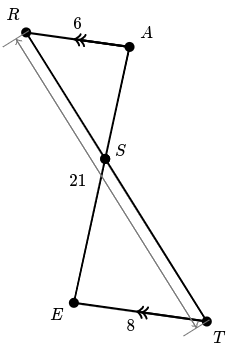
\includegraphics[width =0.9\linewidth ]{Images/triang_sem05}
            \caption{}
            \label{fig:triang_sem05}
        \end{figure}

    \end{minipage}
\end{minipage}